\documentclass[landscape, a4paper, parskip=half, DIV=13]{scrartcl}
\usepackage[top=1.25cm, bottom=1.0cm, left=7cm, right=7cm, marginparwidth=6.0cm, marginparsep=0pt]{geometry}
\usepackage[dvipsnames]{xcolor}
\usepackage{tikz}
\usetikzlibrary{shapes.geometric}
\usepackage{fontspec}
%\setmainfont{Tex Gyre Schola}
\setmainfont[Scale=0.95]{Century Gothic}
\usepackage{contour}
\usepackage{multicol}
\setlength{\columnsep}{1cm}
\usepackage{booktabs}
\usepackage{lipsum}
\usepackage{marginnote}
\usepackage{multirow}
\usepackage{enumitem}
\usepackage{gerrymander}

%\setkomafont{section}{\setmainfont{Tex Gyre Schola}\LARGE\textbf}
\setkomafont{section}{\setmainfont[Scale=0.95]{Century Gothic}\LARGE\textbf}

% Adjust spacing before and after section headings
\RedeclareSectionCommand[
  runin=false,
  beforeskip=1.0\baselineskip,
  afterskip=0.0\baselineskip
]{section}


\pagestyle{empty}
\begin{document}
{
%\setmainfont[Scale=2.5]{Tex Gyre Schola}
\setmainfont[Scale=2.375]{Century Gothic}
\begin{center}
\Huge \textbf{Gerrymander}
\end{center}
}

\vspace{0.0cm}
\vspace{-0.5cm}

\begin{center}
\scalebox{2.85}{
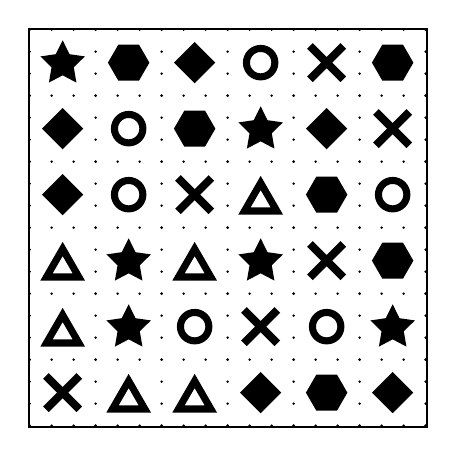
\begin{tikzpicture}
\node[minimum width=0.33in,minimum height=0.33in] at (0.495000in, -0.495000in) {\phantom{.}};
\node[draw=black,circle,inner sep=0.75pt,line width=0.9mm] at (0.495000in, -0.495000in) {\phantom{1}};
\node[minimum width=0.33in,minimum height=0.33in] at (-0.495000in, 0.165000in) {\phantom{.}};
\node[draw=black,circle,inner sep=0.75pt,line width=0.9mm] at (-0.495000in, 0.165000in) {\phantom{1}};
\node[minimum width=0.33in,minimum height=0.33in] at (-0.495000in, 0.495000in) {\phantom{.}};
\node[draw=black,circle,inner sep=0.75pt,line width=0.9mm] at (-0.495000in, 0.495000in) {\phantom{1}};
\node[minimum width=0.33in,minimum height=0.33in] at (-0.165000in, -0.495000in) {\phantom{.}};
\node[draw=black,circle,inner sep=0.75pt,line width=0.9mm] at (-0.165000in, -0.495000in) {\phantom{1}};
\node[minimum width=0.33in,minimum height=0.33in] at (0.165000in, 0.825000in) {\phantom{.}};
\node[draw=black,circle,inner sep=0.75pt,line width=0.9mm] at (0.165000in, 0.825000in) {\phantom{1}};
\node[minimum width=0.33in,minimum height=0.33in] at (0.825000in, 0.165000in) {\phantom{.}};
\node[draw=black,circle,inner sep=0.75pt,line width=0.9mm] at (0.825000in, 0.165000in) {\phantom{1}};
\node[minimum width=0.33in,minimum height=0.33in] at (-0.165000in, 0.165000in) {\phantom{.}};
\node[text=black,rotate=45,inner sep=0pt] at (-0.165000in, 0.165000in) {\rule{6mm}{1mm}};
\node[text=black,rotate=-45,inner sep=0pt] at (-0.165000in, 0.165000in) {\rule{6mm}{1mm}};
\node[minimum width=0.33in,minimum height=0.33in] at (0.495000in, 0.825000in) {\phantom{.}};
\node[text=black,rotate=45,inner sep=0pt] at (0.495000in, 0.825000in) {\rule{6mm}{1mm}};
\node[text=black,rotate=-45,inner sep=0pt] at (0.495000in, 0.825000in) {\rule{6mm}{1mm}};
\node[minimum width=0.33in,minimum height=0.33in] at (0.495000in, -0.165000in) {\phantom{.}};
\node[text=black,rotate=45,inner sep=0pt] at (0.495000in, -0.165000in) {\rule{6mm}{1mm}};
\node[text=black,rotate=-45,inner sep=0pt] at (0.495000in, -0.165000in) {\rule{6mm}{1mm}};
\node[minimum width=0.33in,minimum height=0.33in] at (-0.825000in, -0.825000in) {\phantom{.}};
\node[text=black,rotate=45,inner sep=0pt] at (-0.825000in, -0.825000in) {\rule{6mm}{1mm}};
\node[text=black,rotate=-45,inner sep=0pt] at (-0.825000in, -0.825000in) {\rule{6mm}{1mm}};
\node[minimum width=0.33in,minimum height=0.33in] at (0.165000in, -0.495000in) {\phantom{.}};
\node[text=black,rotate=45,inner sep=0pt] at (0.165000in, -0.495000in) {\rule{6mm}{1mm}};
\node[text=black,rotate=-45,inner sep=0pt] at (0.165000in, -0.495000in) {\rule{6mm}{1mm}};
\node[minimum width=0.33in,minimum height=0.33in] at (0.825000in, 0.495000in) {\phantom{.}};
\node[text=black,rotate=45,inner sep=0pt] at (0.825000in, 0.495000in) {\rule{6mm}{1mm}};
\node[text=black,rotate=-45,inner sep=0pt] at (0.825000in, 0.495000in) {\rule{6mm}{1mm}};
\node[minimum width=0.33in,minimum height=0.33in] at (0.165000in, 0.165000in) {\phantom{.}};
\node[regular polygon,regular polygon sides=3,draw=black,line width=0.9mm,inner sep=1.0pt] at (0.165000in, 0.130000in) {\phantom{.}};
\node[minimum width=0.33in,minimum height=0.33in] at (-0.825000in, -0.495000in) {\phantom{.}};
\node[regular polygon,regular polygon sides=3,draw=black,line width=0.9mm,inner sep=1.0pt] at (-0.825000in, -0.530000in) {\phantom{.}};
\node[minimum width=0.33in,minimum height=0.33in] at (-0.825000in, -0.165000in) {\phantom{.}};
\node[regular polygon,regular polygon sides=3,draw=black,line width=0.9mm,inner sep=1.0pt] at (-0.825000in, -0.200000in) {\phantom{.}};
\node[minimum width=0.33in,minimum height=0.33in] at (-0.165000in, -0.825000in) {\phantom{.}};
\node[regular polygon,regular polygon sides=3,draw=black,line width=0.9mm,inner sep=1.0pt] at (-0.165000in, -0.860000in) {\phantom{.}};
\node[minimum width=0.33in,minimum height=0.33in] at (-0.165000in, -0.165000in) {\phantom{.}};
\node[regular polygon,regular polygon sides=3,draw=black,line width=0.9mm,inner sep=1.0pt] at (-0.165000in, -0.200000in) {\phantom{.}};
\node[minimum width=0.33in,minimum height=0.33in] at (-0.495000in, -0.825000in) {\phantom{.}};
\node[regular polygon,regular polygon sides=3,draw=black,line width=0.9mm,inner sep=1.0pt] at (-0.495000in, -0.860000in) {\phantom{.}};
\node[minimum width=0.33in,minimum height=0.33in] at (0.165000in, -0.825000in) {\phantom{.}};
\node[draw=black,diamond,inner sep=2.125pt,line width=0.9mm,fill=black] at (0.165000in, -0.825000in) {\phantom{.}};
\node[minimum width=0.33in,minimum height=0.33in] at (0.495000in, 0.495000in) {\phantom{.}};
\node[draw=black,diamond,inner sep=2.125pt,line width=0.9mm,fill=black] at (0.495000in, 0.495000in) {\phantom{.}};
\node[minimum width=0.33in,minimum height=0.33in] at (0.825000in, -0.825000in) {\phantom{.}};
\node[draw=black,diamond,inner sep=2.125pt,line width=0.9mm,fill=black] at (0.825000in, -0.825000in) {\phantom{.}};
\node[minimum width=0.33in,minimum height=0.33in] at (-0.825000in, 0.165000in) {\phantom{.}};
\node[draw=black,diamond,inner sep=2.125pt,line width=0.9mm,fill=black] at (-0.825000in, 0.165000in) {\phantom{.}};
\node[minimum width=0.33in,minimum height=0.33in] at (-0.825000in, 0.495000in) {\phantom{.}};
\node[draw=black,diamond,inner sep=2.125pt,line width=0.9mm,fill=black] at (-0.825000in, 0.495000in) {\phantom{.}};
\node[minimum width=0.33in,minimum height=0.33in] at (-0.165000in, 0.825000in) {\phantom{.}};
\node[draw=black,diamond,inner sep=2.125pt,line width=0.9mm,fill=black] at (-0.165000in, 0.825000in) {\phantom{.}};
\node[minimum width=0.33in,minimum height=0.33in] at (-0.825000in, 0.825000in) {\phantom{.}};
\node[star,star points=5,star point ratio=2,fill=black,inner sep=1.6pt] at (-0.825000in, 0.820000in) {\phantom{.}};
\node[minimum width=0.33in,minimum height=0.33in] at (-0.495000in, -0.165000in) {\phantom{.}};
\node[star,star points=5,star point ratio=2,fill=black,inner sep=1.6pt] at (-0.495000in, -0.170000in) {\phantom{.}};
\node[minimum width=0.33in,minimum height=0.33in] at (0.165000in, 0.495000in) {\phantom{.}};
\node[star,star points=5,star point ratio=2,fill=black,inner sep=1.6pt] at (0.165000in, 0.490000in) {\phantom{.}};
\node[minimum width=0.33in,minimum height=0.33in] at (0.165000in, -0.165000in) {\phantom{.}};
\node[star,star points=5,star point ratio=2,fill=black,inner sep=1.6pt] at (0.165000in, -0.170000in) {\phantom{.}};
\node[minimum width=0.33in,minimum height=0.33in] at (-0.495000in, -0.495000in) {\phantom{.}};
\node[star,star points=5,star point ratio=2,fill=black,inner sep=1.6pt] at (-0.495000in, -0.500000in) {\phantom{.}};
\node[minimum width=0.33in,minimum height=0.33in] at (0.825000in, -0.495000in) {\phantom{.}};
\node[star,star points=5,star point ratio=2,fill=black,inner sep=1.6pt] at (0.825000in, -0.500000in) {\phantom{.}};
\node[minimum width=0.33in,minimum height=0.33in] at (0.495000in, -0.825000in) {\phantom{.}};
\node[regular polygon,regular polygon sides=6,fill=black,inner sep=3.2pt] at (0.495000in, -0.825000in) {\phantom{.}};
\node[minimum width=0.33in,minimum height=0.33in] at (0.825000in, -0.165000in) {\phantom{.}};
\node[regular polygon,regular polygon sides=6,fill=black,inner sep=3.2pt] at (0.825000in, -0.165000in) {\phantom{.}};
\node[minimum width=0.33in,minimum height=0.33in] at (0.495000in, 0.165000in) {\phantom{.}};
\node[regular polygon,regular polygon sides=6,fill=black,inner sep=3.2pt] at (0.495000in, 0.165000in) {\phantom{.}};
\node[minimum width=0.33in,minimum height=0.33in] at (-0.165000in, 0.495000in) {\phantom{.}};
\node[regular polygon,regular polygon sides=6,fill=black,inner sep=3.2pt] at (-0.165000in, 0.495000in) {\phantom{.}};
\node[minimum width=0.33in,minimum height=0.33in] at (-0.495000in, 0.825000in) {\phantom{.}};
\node[regular polygon,regular polygon sides=6,fill=black,inner sep=3.2pt] at (-0.495000in, 0.825000in) {\phantom{.}};
\node[minimum width=0.33in,minimum height=0.33in] at (0.825000in, 0.825000in) {\phantom{.}};
\node[regular polygon,regular polygon sides=6,fill=black,inner sep=3.2pt] at (0.825000in, 0.825000in) {\phantom{.}};
\node[inner sep=0.25pt,fill=black,circle] at (-0.990000in, -0.990000in) {\phantom{}};
\node[inner sep=0.25pt,fill=black,circle] at (-0.990000in, -0.660000in) {\phantom{}};
\node[inner sep=0.25pt,fill=black,circle] at (-0.990000in, -0.330000in) {\phantom{}};
\node[inner sep=0.25pt,fill=black,circle] at (-0.990000in, 0.000000in) {\phantom{}};
\node[inner sep=0.25pt,fill=black,circle] at (-0.990000in, 0.330000in) {\phantom{}};
\node[inner sep=0.25pt,fill=black,circle] at (-0.990000in, 0.660000in) {\phantom{}};
\node[inner sep=0.25pt,fill=black,circle] at (-0.990000in, 0.990000in) {\phantom{}};
\node[inner sep=0.25pt,fill=black,circle] at (-0.880000in, -0.990000in) {\phantom{}};
\node[inner sep=0.25pt,fill=black,circle] at (-0.880000in, -0.660000in) {\phantom{}};
\node[inner sep=0.25pt,fill=black,circle] at (-0.880000in, -0.330000in) {\phantom{}};
\node[inner sep=0.25pt,fill=black,circle] at (-0.880000in, 0.000000in) {\phantom{}};
\node[inner sep=0.25pt,fill=black,circle] at (-0.880000in, 0.330000in) {\phantom{}};
\node[inner sep=0.25pt,fill=black,circle] at (-0.880000in, 0.660000in) {\phantom{}};
\node[inner sep=0.25pt,fill=black,circle] at (-0.880000in, 0.990000in) {\phantom{}};
\node[inner sep=0.25pt,fill=black,circle] at (-0.770000in, -0.990000in) {\phantom{}};
\node[inner sep=0.25pt,fill=black,circle] at (-0.770000in, -0.660000in) {\phantom{}};
\node[inner sep=0.25pt,fill=black,circle] at (-0.770000in, -0.330000in) {\phantom{}};
\node[inner sep=0.25pt,fill=black,circle] at (-0.770000in, 0.000000in) {\phantom{}};
\node[inner sep=0.25pt,fill=black,circle] at (-0.770000in, 0.330000in) {\phantom{}};
\node[inner sep=0.25pt,fill=black,circle] at (-0.770000in, 0.660000in) {\phantom{}};
\node[inner sep=0.25pt,fill=black,circle] at (-0.770000in, 0.990000in) {\phantom{}};
\node[inner sep=0.25pt,fill=black,circle] at (-0.660000in, -0.990000in) {\phantom{}};
\node[inner sep=0.25pt,fill=black,circle] at (-0.660000in, -0.660000in) {\phantom{}};
\node[inner sep=0.25pt,fill=black,circle] at (-0.660000in, -0.330000in) {\phantom{}};
\node[inner sep=0.25pt,fill=black,circle] at (-0.660000in, 0.000000in) {\phantom{}};
\node[inner sep=0.25pt,fill=black,circle] at (-0.660000in, 0.330000in) {\phantom{}};
\node[inner sep=0.25pt,fill=black,circle] at (-0.660000in, 0.660000in) {\phantom{}};
\node[inner sep=0.25pt,fill=black,circle] at (-0.660000in, 0.990000in) {\phantom{}};
\node[inner sep=0.25pt,fill=black,circle] at (-0.550000in, -0.990000in) {\phantom{}};
\node[inner sep=0.25pt,fill=black,circle] at (-0.550000in, -0.660000in) {\phantom{}};
\node[inner sep=0.25pt,fill=black,circle] at (-0.550000in, -0.330000in) {\phantom{}};
\node[inner sep=0.25pt,fill=black,circle] at (-0.550000in, 0.000000in) {\phantom{}};
\node[inner sep=0.25pt,fill=black,circle] at (-0.550000in, 0.330000in) {\phantom{}};
\node[inner sep=0.25pt,fill=black,circle] at (-0.550000in, 0.660000in) {\phantom{}};
\node[inner sep=0.25pt,fill=black,circle] at (-0.550000in, 0.990000in) {\phantom{}};
\node[inner sep=0.25pt,fill=black,circle] at (-0.440000in, -0.990000in) {\phantom{}};
\node[inner sep=0.25pt,fill=black,circle] at (-0.440000in, -0.660000in) {\phantom{}};
\node[inner sep=0.25pt,fill=black,circle] at (-0.440000in, -0.330000in) {\phantom{}};
\node[inner sep=0.25pt,fill=black,circle] at (-0.440000in, 0.000000in) {\phantom{}};
\node[inner sep=0.25pt,fill=black,circle] at (-0.440000in, 0.330000in) {\phantom{}};
\node[inner sep=0.25pt,fill=black,circle] at (-0.440000in, 0.660000in) {\phantom{}};
\node[inner sep=0.25pt,fill=black,circle] at (-0.440000in, 0.990000in) {\phantom{}};
\node[inner sep=0.25pt,fill=black,circle] at (-0.330000in, -0.990000in) {\phantom{}};
\node[inner sep=0.25pt,fill=black,circle] at (-0.330000in, -0.660000in) {\phantom{}};
\node[inner sep=0.25pt,fill=black,circle] at (-0.330000in, -0.330000in) {\phantom{}};
\node[inner sep=0.25pt,fill=black,circle] at (-0.330000in, 0.000000in) {\phantom{}};
\node[inner sep=0.25pt,fill=black,circle] at (-0.330000in, 0.330000in) {\phantom{}};
\node[inner sep=0.25pt,fill=black,circle] at (-0.330000in, 0.660000in) {\phantom{}};
\node[inner sep=0.25pt,fill=black,circle] at (-0.330000in, 0.990000in) {\phantom{}};
\node[inner sep=0.25pt,fill=black,circle] at (-0.220000in, -0.990000in) {\phantom{}};
\node[inner sep=0.25pt,fill=black,circle] at (-0.220000in, -0.660000in) {\phantom{}};
\node[inner sep=0.25pt,fill=black,circle] at (-0.220000in, -0.330000in) {\phantom{}};
\node[inner sep=0.25pt,fill=black,circle] at (-0.220000in, 0.000000in) {\phantom{}};
\node[inner sep=0.25pt,fill=black,circle] at (-0.220000in, 0.330000in) {\phantom{}};
\node[inner sep=0.25pt,fill=black,circle] at (-0.220000in, 0.660000in) {\phantom{}};
\node[inner sep=0.25pt,fill=black,circle] at (-0.220000in, 0.990000in) {\phantom{}};
\node[inner sep=0.25pt,fill=black,circle] at (-0.110000in, -0.990000in) {\phantom{}};
\node[inner sep=0.25pt,fill=black,circle] at (-0.110000in, -0.660000in) {\phantom{}};
\node[inner sep=0.25pt,fill=black,circle] at (-0.110000in, -0.330000in) {\phantom{}};
\node[inner sep=0.25pt,fill=black,circle] at (-0.110000in, 0.000000in) {\phantom{}};
\node[inner sep=0.25pt,fill=black,circle] at (-0.110000in, 0.330000in) {\phantom{}};
\node[inner sep=0.25pt,fill=black,circle] at (-0.110000in, 0.660000in) {\phantom{}};
\node[inner sep=0.25pt,fill=black,circle] at (-0.110000in, 0.990000in) {\phantom{}};
\node[inner sep=0.25pt,fill=black,circle] at (-0.000000in, -0.990000in) {\phantom{}};
\node[inner sep=0.25pt,fill=black,circle] at (-0.000000in, -0.660000in) {\phantom{}};
\node[inner sep=0.25pt,fill=black,circle] at (-0.000000in, -0.330000in) {\phantom{}};
\node[inner sep=0.25pt,fill=black,circle] at (-0.000000in, 0.000000in) {\phantom{}};
\node[inner sep=0.25pt,fill=black,circle] at (-0.000000in, 0.330000in) {\phantom{}};
\node[inner sep=0.25pt,fill=black,circle] at (-0.000000in, 0.660000in) {\phantom{}};
\node[inner sep=0.25pt,fill=black,circle] at (-0.000000in, 0.990000in) {\phantom{}};
\node[inner sep=0.25pt,fill=black,circle] at (0.110000in, -0.990000in) {\phantom{}};
\node[inner sep=0.25pt,fill=black,circle] at (0.110000in, -0.660000in) {\phantom{}};
\node[inner sep=0.25pt,fill=black,circle] at (0.110000in, -0.330000in) {\phantom{}};
\node[inner sep=0.25pt,fill=black,circle] at (0.110000in, 0.000000in) {\phantom{}};
\node[inner sep=0.25pt,fill=black,circle] at (0.110000in, 0.330000in) {\phantom{}};
\node[inner sep=0.25pt,fill=black,circle] at (0.110000in, 0.660000in) {\phantom{}};
\node[inner sep=0.25pt,fill=black,circle] at (0.110000in, 0.990000in) {\phantom{}};
\node[inner sep=0.25pt,fill=black,circle] at (0.220000in, -0.990000in) {\phantom{}};
\node[inner sep=0.25pt,fill=black,circle] at (0.220000in, -0.660000in) {\phantom{}};
\node[inner sep=0.25pt,fill=black,circle] at (0.220000in, -0.330000in) {\phantom{}};
\node[inner sep=0.25pt,fill=black,circle] at (0.220000in, 0.000000in) {\phantom{}};
\node[inner sep=0.25pt,fill=black,circle] at (0.220000in, 0.330000in) {\phantom{}};
\node[inner sep=0.25pt,fill=black,circle] at (0.220000in, 0.660000in) {\phantom{}};
\node[inner sep=0.25pt,fill=black,circle] at (0.220000in, 0.990000in) {\phantom{}};
\node[inner sep=0.25pt,fill=black,circle] at (0.330000in, -0.990000in) {\phantom{}};
\node[inner sep=0.25pt,fill=black,circle] at (0.330000in, -0.660000in) {\phantom{}};
\node[inner sep=0.25pt,fill=black,circle] at (0.330000in, -0.330000in) {\phantom{}};
\node[inner sep=0.25pt,fill=black,circle] at (0.330000in, 0.000000in) {\phantom{}};
\node[inner sep=0.25pt,fill=black,circle] at (0.330000in, 0.330000in) {\phantom{}};
\node[inner sep=0.25pt,fill=black,circle] at (0.330000in, 0.660000in) {\phantom{}};
\node[inner sep=0.25pt,fill=black,circle] at (0.330000in, 0.990000in) {\phantom{}};
\node[inner sep=0.25pt,fill=black,circle] at (0.440000in, -0.990000in) {\phantom{}};
\node[inner sep=0.25pt,fill=black,circle] at (0.440000in, -0.660000in) {\phantom{}};
\node[inner sep=0.25pt,fill=black,circle] at (0.440000in, -0.330000in) {\phantom{}};
\node[inner sep=0.25pt,fill=black,circle] at (0.440000in, 0.000000in) {\phantom{}};
\node[inner sep=0.25pt,fill=black,circle] at (0.440000in, 0.330000in) {\phantom{}};
\node[inner sep=0.25pt,fill=black,circle] at (0.440000in, 0.660000in) {\phantom{}};
\node[inner sep=0.25pt,fill=black,circle] at (0.440000in, 0.990000in) {\phantom{}};
\node[inner sep=0.25pt,fill=black,circle] at (0.550000in, -0.990000in) {\phantom{}};
\node[inner sep=0.25pt,fill=black,circle] at (0.550000in, -0.660000in) {\phantom{}};
\node[inner sep=0.25pt,fill=black,circle] at (0.550000in, -0.330000in) {\phantom{}};
\node[inner sep=0.25pt,fill=black,circle] at (0.550000in, 0.000000in) {\phantom{}};
\node[inner sep=0.25pt,fill=black,circle] at (0.550000in, 0.330000in) {\phantom{}};
\node[inner sep=0.25pt,fill=black,circle] at (0.550000in, 0.660000in) {\phantom{}};
\node[inner sep=0.25pt,fill=black,circle] at (0.550000in, 0.990000in) {\phantom{}};
\node[inner sep=0.25pt,fill=black,circle] at (0.660000in, -0.990000in) {\phantom{}};
\node[inner sep=0.25pt,fill=black,circle] at (0.660000in, -0.660000in) {\phantom{}};
\node[inner sep=0.25pt,fill=black,circle] at (0.660000in, -0.330000in) {\phantom{}};
\node[inner sep=0.25pt,fill=black,circle] at (0.660000in, 0.000000in) {\phantom{}};
\node[inner sep=0.25pt,fill=black,circle] at (0.660000in, 0.330000in) {\phantom{}};
\node[inner sep=0.25pt,fill=black,circle] at (0.660000in, 0.660000in) {\phantom{}};
\node[inner sep=0.25pt,fill=black,circle] at (0.660000in, 0.990000in) {\phantom{}};
\node[inner sep=0.25pt,fill=black,circle] at (0.770000in, -0.990000in) {\phantom{}};
\node[inner sep=0.25pt,fill=black,circle] at (0.770000in, -0.660000in) {\phantom{}};
\node[inner sep=0.25pt,fill=black,circle] at (0.770000in, -0.330000in) {\phantom{}};
\node[inner sep=0.25pt,fill=black,circle] at (0.770000in, 0.000000in) {\phantom{}};
\node[inner sep=0.25pt,fill=black,circle] at (0.770000in, 0.330000in) {\phantom{}};
\node[inner sep=0.25pt,fill=black,circle] at (0.770000in, 0.660000in) {\phantom{}};
\node[inner sep=0.25pt,fill=black,circle] at (0.770000in, 0.990000in) {\phantom{}};
\node[inner sep=0.25pt,fill=black,circle] at (0.880000in, -0.990000in) {\phantom{}};
\node[inner sep=0.25pt,fill=black,circle] at (0.880000in, -0.660000in) {\phantom{}};
\node[inner sep=0.25pt,fill=black,circle] at (0.880000in, -0.330000in) {\phantom{}};
\node[inner sep=0.25pt,fill=black,circle] at (0.880000in, 0.000000in) {\phantom{}};
\node[inner sep=0.25pt,fill=black,circle] at (0.880000in, 0.330000in) {\phantom{}};
\node[inner sep=0.25pt,fill=black,circle] at (0.880000in, 0.660000in) {\phantom{}};
\node[inner sep=0.25pt,fill=black,circle] at (0.880000in, 0.990000in) {\phantom{}};
\node[inner sep=0.25pt,fill=black,circle] at (0.990000in, -0.990000in) {\phantom{}};
\node[inner sep=0.25pt,fill=black,circle] at (0.990000in, -0.660000in) {\phantom{}};
\node[inner sep=0.25pt,fill=black,circle] at (0.990000in, -0.330000in) {\phantom{}};
\node[inner sep=0.25pt,fill=black,circle] at (0.990000in, 0.000000in) {\phantom{}};
\node[inner sep=0.25pt,fill=black,circle] at (0.990000in, 0.330000in) {\phantom{}};
\node[inner sep=0.25pt,fill=black,circle] at (0.990000in, 0.660000in) {\phantom{}};
\node[inner sep=0.25pt,fill=black,circle] at (0.990000in, 0.990000in) {\phantom{}};
\node[inner sep=0.25pt,fill=black,circle] at (-0.990000in, -0.990000in) {\phantom{}};
\node[inner sep=0.25pt,fill=black,circle] at (-0.990000in, -0.880000in) {\phantom{}};
\node[inner sep=0.25pt,fill=black,circle] at (-0.990000in, -0.770000in) {\phantom{}};
\node[inner sep=0.25pt,fill=black,circle] at (-0.990000in, -0.660000in) {\phantom{}};
\node[inner sep=0.25pt,fill=black,circle] at (-0.990000in, -0.550000in) {\phantom{}};
\node[inner sep=0.25pt,fill=black,circle] at (-0.990000in, -0.440000in) {\phantom{}};
\node[inner sep=0.25pt,fill=black,circle] at (-0.990000in, -0.330000in) {\phantom{}};
\node[inner sep=0.25pt,fill=black,circle] at (-0.990000in, -0.220000in) {\phantom{}};
\node[inner sep=0.25pt,fill=black,circle] at (-0.990000in, -0.110000in) {\phantom{}};
\node[inner sep=0.25pt,fill=black,circle] at (-0.990000in, -0.000000in) {\phantom{}};
\node[inner sep=0.25pt,fill=black,circle] at (-0.990000in, 0.110000in) {\phantom{}};
\node[inner sep=0.25pt,fill=black,circle] at (-0.990000in, 0.220000in) {\phantom{}};
\node[inner sep=0.25pt,fill=black,circle] at (-0.990000in, 0.330000in) {\phantom{}};
\node[inner sep=0.25pt,fill=black,circle] at (-0.990000in, 0.440000in) {\phantom{}};
\node[inner sep=0.25pt,fill=black,circle] at (-0.990000in, 0.550000in) {\phantom{}};
\node[inner sep=0.25pt,fill=black,circle] at (-0.990000in, 0.660000in) {\phantom{}};
\node[inner sep=0.25pt,fill=black,circle] at (-0.990000in, 0.770000in) {\phantom{}};
\node[inner sep=0.25pt,fill=black,circle] at (-0.990000in, 0.880000in) {\phantom{}};
\node[inner sep=0.25pt,fill=black,circle] at (-0.990000in, 0.990000in) {\phantom{}};
\node[inner sep=0.25pt,fill=black,circle] at (-0.660000in, -0.990000in) {\phantom{}};
\node[inner sep=0.25pt,fill=black,circle] at (-0.660000in, -0.880000in) {\phantom{}};
\node[inner sep=0.25pt,fill=black,circle] at (-0.660000in, -0.770000in) {\phantom{}};
\node[inner sep=0.25pt,fill=black,circle] at (-0.660000in, -0.660000in) {\phantom{}};
\node[inner sep=0.25pt,fill=black,circle] at (-0.660000in, -0.550000in) {\phantom{}};
\node[inner sep=0.25pt,fill=black,circle] at (-0.660000in, -0.440000in) {\phantom{}};
\node[inner sep=0.25pt,fill=black,circle] at (-0.660000in, -0.330000in) {\phantom{}};
\node[inner sep=0.25pt,fill=black,circle] at (-0.660000in, -0.220000in) {\phantom{}};
\node[inner sep=0.25pt,fill=black,circle] at (-0.660000in, -0.110000in) {\phantom{}};
\node[inner sep=0.25pt,fill=black,circle] at (-0.660000in, -0.000000in) {\phantom{}};
\node[inner sep=0.25pt,fill=black,circle] at (-0.660000in, 0.110000in) {\phantom{}};
\node[inner sep=0.25pt,fill=black,circle] at (-0.660000in, 0.220000in) {\phantom{}};
\node[inner sep=0.25pt,fill=black,circle] at (-0.660000in, 0.330000in) {\phantom{}};
\node[inner sep=0.25pt,fill=black,circle] at (-0.660000in, 0.440000in) {\phantom{}};
\node[inner sep=0.25pt,fill=black,circle] at (-0.660000in, 0.550000in) {\phantom{}};
\node[inner sep=0.25pt,fill=black,circle] at (-0.660000in, 0.660000in) {\phantom{}};
\node[inner sep=0.25pt,fill=black,circle] at (-0.660000in, 0.770000in) {\phantom{}};
\node[inner sep=0.25pt,fill=black,circle] at (-0.660000in, 0.880000in) {\phantom{}};
\node[inner sep=0.25pt,fill=black,circle] at (-0.660000in, 0.990000in) {\phantom{}};
\node[inner sep=0.25pt,fill=black,circle] at (-0.330000in, -0.990000in) {\phantom{}};
\node[inner sep=0.25pt,fill=black,circle] at (-0.330000in, -0.880000in) {\phantom{}};
\node[inner sep=0.25pt,fill=black,circle] at (-0.330000in, -0.770000in) {\phantom{}};
\node[inner sep=0.25pt,fill=black,circle] at (-0.330000in, -0.660000in) {\phantom{}};
\node[inner sep=0.25pt,fill=black,circle] at (-0.330000in, -0.550000in) {\phantom{}};
\node[inner sep=0.25pt,fill=black,circle] at (-0.330000in, -0.440000in) {\phantom{}};
\node[inner sep=0.25pt,fill=black,circle] at (-0.330000in, -0.330000in) {\phantom{}};
\node[inner sep=0.25pt,fill=black,circle] at (-0.330000in, -0.220000in) {\phantom{}};
\node[inner sep=0.25pt,fill=black,circle] at (-0.330000in, -0.110000in) {\phantom{}};
\node[inner sep=0.25pt,fill=black,circle] at (-0.330000in, -0.000000in) {\phantom{}};
\node[inner sep=0.25pt,fill=black,circle] at (-0.330000in, 0.110000in) {\phantom{}};
\node[inner sep=0.25pt,fill=black,circle] at (-0.330000in, 0.220000in) {\phantom{}};
\node[inner sep=0.25pt,fill=black,circle] at (-0.330000in, 0.330000in) {\phantom{}};
\node[inner sep=0.25pt,fill=black,circle] at (-0.330000in, 0.440000in) {\phantom{}};
\node[inner sep=0.25pt,fill=black,circle] at (-0.330000in, 0.550000in) {\phantom{}};
\node[inner sep=0.25pt,fill=black,circle] at (-0.330000in, 0.660000in) {\phantom{}};
\node[inner sep=0.25pt,fill=black,circle] at (-0.330000in, 0.770000in) {\phantom{}};
\node[inner sep=0.25pt,fill=black,circle] at (-0.330000in, 0.880000in) {\phantom{}};
\node[inner sep=0.25pt,fill=black,circle] at (-0.330000in, 0.990000in) {\phantom{}};
\node[inner sep=0.25pt,fill=black,circle] at (0.000000in, -0.990000in) {\phantom{}};
\node[inner sep=0.25pt,fill=black,circle] at (0.000000in, -0.880000in) {\phantom{}};
\node[inner sep=0.25pt,fill=black,circle] at (0.000000in, -0.770000in) {\phantom{}};
\node[inner sep=0.25pt,fill=black,circle] at (0.000000in, -0.660000in) {\phantom{}};
\node[inner sep=0.25pt,fill=black,circle] at (0.000000in, -0.550000in) {\phantom{}};
\node[inner sep=0.25pt,fill=black,circle] at (0.000000in, -0.440000in) {\phantom{}};
\node[inner sep=0.25pt,fill=black,circle] at (0.000000in, -0.330000in) {\phantom{}};
\node[inner sep=0.25pt,fill=black,circle] at (0.000000in, -0.220000in) {\phantom{}};
\node[inner sep=0.25pt,fill=black,circle] at (0.000000in, -0.110000in) {\phantom{}};
\node[inner sep=0.25pt,fill=black,circle] at (0.000000in, -0.000000in) {\phantom{}};
\node[inner sep=0.25pt,fill=black,circle] at (0.000000in, 0.110000in) {\phantom{}};
\node[inner sep=0.25pt,fill=black,circle] at (0.000000in, 0.220000in) {\phantom{}};
\node[inner sep=0.25pt,fill=black,circle] at (0.000000in, 0.330000in) {\phantom{}};
\node[inner sep=0.25pt,fill=black,circle] at (0.000000in, 0.440000in) {\phantom{}};
\node[inner sep=0.25pt,fill=black,circle] at (0.000000in, 0.550000in) {\phantom{}};
\node[inner sep=0.25pt,fill=black,circle] at (0.000000in, 0.660000in) {\phantom{}};
\node[inner sep=0.25pt,fill=black,circle] at (0.000000in, 0.770000in) {\phantom{}};
\node[inner sep=0.25pt,fill=black,circle] at (0.000000in, 0.880000in) {\phantom{}};
\node[inner sep=0.25pt,fill=black,circle] at (0.000000in, 0.990000in) {\phantom{}};
\node[inner sep=0.25pt,fill=black,circle] at (0.330000in, -0.990000in) {\phantom{}};
\node[inner sep=0.25pt,fill=black,circle] at (0.330000in, -0.880000in) {\phantom{}};
\node[inner sep=0.25pt,fill=black,circle] at (0.330000in, -0.770000in) {\phantom{}};
\node[inner sep=0.25pt,fill=black,circle] at (0.330000in, -0.660000in) {\phantom{}};
\node[inner sep=0.25pt,fill=black,circle] at (0.330000in, -0.550000in) {\phantom{}};
\node[inner sep=0.25pt,fill=black,circle] at (0.330000in, -0.440000in) {\phantom{}};
\node[inner sep=0.25pt,fill=black,circle] at (0.330000in, -0.330000in) {\phantom{}};
\node[inner sep=0.25pt,fill=black,circle] at (0.330000in, -0.220000in) {\phantom{}};
\node[inner sep=0.25pt,fill=black,circle] at (0.330000in, -0.110000in) {\phantom{}};
\node[inner sep=0.25pt,fill=black,circle] at (0.330000in, -0.000000in) {\phantom{}};
\node[inner sep=0.25pt,fill=black,circle] at (0.330000in, 0.110000in) {\phantom{}};
\node[inner sep=0.25pt,fill=black,circle] at (0.330000in, 0.220000in) {\phantom{}};
\node[inner sep=0.25pt,fill=black,circle] at (0.330000in, 0.330000in) {\phantom{}};
\node[inner sep=0.25pt,fill=black,circle] at (0.330000in, 0.440000in) {\phantom{}};
\node[inner sep=0.25pt,fill=black,circle] at (0.330000in, 0.550000in) {\phantom{}};
\node[inner sep=0.25pt,fill=black,circle] at (0.330000in, 0.660000in) {\phantom{}};
\node[inner sep=0.25pt,fill=black,circle] at (0.330000in, 0.770000in) {\phantom{}};
\node[inner sep=0.25pt,fill=black,circle] at (0.330000in, 0.880000in) {\phantom{}};
\node[inner sep=0.25pt,fill=black,circle] at (0.330000in, 0.990000in) {\phantom{}};
\node[inner sep=0.25pt,fill=black,circle] at (0.660000in, -0.990000in) {\phantom{}};
\node[inner sep=0.25pt,fill=black,circle] at (0.660000in, -0.880000in) {\phantom{}};
\node[inner sep=0.25pt,fill=black,circle] at (0.660000in, -0.770000in) {\phantom{}};
\node[inner sep=0.25pt,fill=black,circle] at (0.660000in, -0.660000in) {\phantom{}};
\node[inner sep=0.25pt,fill=black,circle] at (0.660000in, -0.550000in) {\phantom{}};
\node[inner sep=0.25pt,fill=black,circle] at (0.660000in, -0.440000in) {\phantom{}};
\node[inner sep=0.25pt,fill=black,circle] at (0.660000in, -0.330000in) {\phantom{}};
\node[inner sep=0.25pt,fill=black,circle] at (0.660000in, -0.220000in) {\phantom{}};
\node[inner sep=0.25pt,fill=black,circle] at (0.660000in, -0.110000in) {\phantom{}};
\node[inner sep=0.25pt,fill=black,circle] at (0.660000in, -0.000000in) {\phantom{}};
\node[inner sep=0.25pt,fill=black,circle] at (0.660000in, 0.110000in) {\phantom{}};
\node[inner sep=0.25pt,fill=black,circle] at (0.660000in, 0.220000in) {\phantom{}};
\node[inner sep=0.25pt,fill=black,circle] at (0.660000in, 0.330000in) {\phantom{}};
\node[inner sep=0.25pt,fill=black,circle] at (0.660000in, 0.440000in) {\phantom{}};
\node[inner sep=0.25pt,fill=black,circle] at (0.660000in, 0.550000in) {\phantom{}};
\node[inner sep=0.25pt,fill=black,circle] at (0.660000in, 0.660000in) {\phantom{}};
\node[inner sep=0.25pt,fill=black,circle] at (0.660000in, 0.770000in) {\phantom{}};
\node[inner sep=0.25pt,fill=black,circle] at (0.660000in, 0.880000in) {\phantom{}};
\node[inner sep=0.25pt,fill=black,circle] at (0.660000in, 0.990000in) {\phantom{}};
\node[inner sep=0.25pt,fill=black,circle] at (0.990000in, -0.990000in) {\phantom{}};
\node[inner sep=0.25pt,fill=black,circle] at (0.990000in, -0.880000in) {\phantom{}};
\node[inner sep=0.25pt,fill=black,circle] at (0.990000in, -0.770000in) {\phantom{}};
\node[inner sep=0.25pt,fill=black,circle] at (0.990000in, -0.660000in) {\phantom{}};
\node[inner sep=0.25pt,fill=black,circle] at (0.990000in, -0.550000in) {\phantom{}};
\node[inner sep=0.25pt,fill=black,circle] at (0.990000in, -0.440000in) {\phantom{}};
\node[inner sep=0.25pt,fill=black,circle] at (0.990000in, -0.330000in) {\phantom{}};
\node[inner sep=0.25pt,fill=black,circle] at (0.990000in, -0.220000in) {\phantom{}};
\node[inner sep=0.25pt,fill=black,circle] at (0.990000in, -0.110000in) {\phantom{}};
\node[inner sep=0.25pt,fill=black,circle] at (0.990000in, -0.000000in) {\phantom{}};
\node[inner sep=0.25pt,fill=black,circle] at (0.990000in, 0.110000in) {\phantom{}};
\node[inner sep=0.25pt,fill=black,circle] at (0.990000in, 0.220000in) {\phantom{}};
\node[inner sep=0.25pt,fill=black,circle] at (0.990000in, 0.330000in) {\phantom{}};
\node[inner sep=0.25pt,fill=black,circle] at (0.990000in, 0.440000in) {\phantom{}};
\node[inner sep=0.25pt,fill=black,circle] at (0.990000in, 0.550000in) {\phantom{}};
\node[inner sep=0.25pt,fill=black,circle] at (0.990000in, 0.660000in) {\phantom{}};
\node[inner sep=0.25pt,fill=black,circle] at (0.990000in, 0.770000in) {\phantom{}};
\node[inner sep=0.25pt,fill=black,circle] at (0.990000in, 0.880000in) {\phantom{}};
\node[inner sep=0.25pt,fill=black,circle] at (0.990000in, 0.990000in) {\phantom{}};
\node[draw,line width=0.25mm,minimum width=1.99in,minimum height=1.99in] at (0in,0in) {\phantom{}};
\end{tikzpicture}
}
\marginnote{\section*{Scoring}
The game ends when you have created nine districts. Your score depends on how many of each icon are in each district.

Consider the scoring table below. For each row you accessed:
\begin{itemize}[leftmargin=*, nosep]
\item Score one point for each of your districts that has three or more of the circled icons.
\vspace{0.2ex}
\item Lose one point for each district that has one or fewer of the circled icons.
\end{itemize}

\vspace{-0.4ex}

\begin{center}
\begin{tabular}{c c@{\hskip 3pt}c@{\hskip 3pt}c c c@{\hskip 3pt}c@{\hskip 3pt}c}\toprule
Die & \multicolumn{3}{c}{Icons} & Die & \multicolumn{3}{c}{Icons} \\ \midrule
\phantom{1}1 & \raisebox{-0.25ex}{\drawonestar{}} & \raisebox{-0.25ex}{\drawtwostar{}} & \raisebox{-0.25ex}{\drawthreestar{}} & 11 & \raisebox{-0.25ex}{\drawfourstar{}} & \raisebox{-0.25ex}{\drawfivestar{}} & \raisebox{-0.25ex}{\drawsixstar{}} \\[0.5ex]
\phantom{1}2 & \raisebox{-0.25ex}{\drawonestar{}} & \raisebox{-0.25ex}{\drawtwostar{}} & \raisebox{-0.25ex}{\drawfourstar{}} & 12 & \raisebox{-0.25ex}{\drawthreestar{}} & \raisebox{-0.25ex}{\drawfivestar{}} & \raisebox{-0.25ex}{\drawsixstar{}} \\[0.5ex]
\phantom{1}3 & \raisebox{-0.25ex}{\drawonestar{}} & \raisebox{-0.25ex}{\drawtwostar{}} & \raisebox{-0.25ex}{\drawfivestar{}} & 13 & \raisebox{-0.25ex}{\drawthreestar{}} & \raisebox{-0.25ex}{\drawfourstar{}} & \raisebox{-0.25ex}{\drawsixstar{}} \\[0.5ex]
\phantom{1}4 & \raisebox{-0.25ex}{\drawonestar{}} & \raisebox{-0.25ex}{\drawtwostar{}} & \raisebox{-0.25ex}{\drawsixstar{}} & 14 & \raisebox{-0.25ex}{\drawthreestar{}} & \raisebox{-0.25ex}{\drawfourstar{}} & \raisebox{-0.25ex}{\drawfivestar{}} \\[0.5ex]
\phantom{1}5 & \raisebox{-0.25ex}{\drawonestar{}} & \raisebox{-0.25ex}{\drawthreestar{}} & \raisebox{-0.25ex}{\drawfourstar{}} & 15 & \raisebox{-0.25ex}{\drawtwostar{}} & \raisebox{-0.25ex}{\drawfivestar{}} & \raisebox{-0.25ex}{\drawsixstar{}} \\[0.5ex]
\phantom{1}6 & \raisebox{-0.25ex}{\drawonestar{}} & \raisebox{-0.25ex}{\drawthreestar{}} & \raisebox{-0.25ex}{\drawfivestar{}} & 16 & \raisebox{-0.25ex}{\drawtwostar{}} & \raisebox{-0.25ex}{\drawfourstar{}} & \raisebox{-0.25ex}{\drawsixstar{}} \\[0.5ex]
\phantom{1}7 & \raisebox{-0.25ex}{\drawonestar{}} & \raisebox{-0.25ex}{\drawthreestar{}} & \raisebox{-0.25ex}{\drawsixstar{}} & 17 & \raisebox{-0.25ex}{\drawtwostar{}} & \raisebox{-0.25ex}{\drawfourstar{}} & \raisebox{-0.25ex}{\drawfivestar{}} \\[0.5ex]
\phantom{1}8 & \raisebox{-0.25ex}{\drawonestar{}} & \raisebox{-0.25ex}{\drawfourstar{}} & \raisebox{-0.25ex}{\drawfivestar{}} & 18 & \raisebox{-0.25ex}{\drawtwostar{}} & \raisebox{-0.25ex}{\drawthreestar{}} & \raisebox{-0.25ex}{\drawsixstar{}} \\[0.5ex]
\phantom{1}9 & \raisebox{-0.25ex}{\drawonestar{}} & \raisebox{-0.25ex}{\drawfourstar{}} & \raisebox{-0.25ex}{\drawsixstar{}} & 19 & \raisebox{-0.25ex}{\drawtwostar{}} & \raisebox{-0.25ex}{\drawthreestar{}} & \raisebox{-0.25ex}{\drawfivestar{}} \\[0.5ex]
10 & \raisebox{-0.25ex}{\drawonestar{}} & \raisebox{-0.25ex}{\drawfivestar{}} & \raisebox{-0.25ex}{\drawsixstar{}} & 20 & \raisebox{-0.25ex}{\drawtwostar{}} & \raisebox{-0.25ex}{\drawthreestar{}} & \raisebox{-0.25ex}{\drawfourstar{}} \\ \bottomrule

\end{tabular}
\end{center}

}[-15.5cm]
\reversemarginpar\marginnote{\raggedright\section*{Gameplay}
Give everyone a pencil and a copy of these rules. Find one 20-sided die to share.

During the game, you will divide your board into nine sets of four grid squares called \emph{districts}. 

Each round, one player should roll the die. Find the row on the scoring table indicated by the die result and do the following:
\begin{itemize}[leftmargin=*, nosep]
\item If you have accessed this row before, then skip this step.
\vspace{0.2ex}
\item Otherwise, circle the icons next to your die result and cross out the other icons on that row.
\end{itemize}

Then, draw a straight line on the board subject to the following:
\begin{itemize}[leftmargin=*, nosep]
\item Your line must start and end at a corner of a grid square.
\vspace{0.2ex}
\item Your line must be either vertical or horizontal.
\vspace{0.2ex}
\item Your line may not pass through another line.
\vspace{0.2ex}
\item Your line may not enclose any regions that do not contain a multiple of four grid squares.
\end{itemize}
}[-15.5cm]

\vfill

{\LARGE Designed by Michael Purcell}
\normalmarginpar\marginnote{\raggedright\textbf{Random Seed}: 983291822}
\reversemarginpar\marginnote{\raggedright\textbf{Contact}: ttkttkt@gmail.com}
\end{center}
\end{document}
